\def\year{2019}\relax
%File: formatting-instruction.tex
\documentclass[letterpaper]{article} %DO NOT CHANGE THIS
\usepackage{aaai19}  %Required
\usepackage{times}  %Required
\usepackage{helvet}  %Required
\usepackage{courier}  %Required
\usepackage{url}  %Required
\usepackage{graphicx}  %Required
%\usepackage{parskip}
\usepackage{algorithm}
\usepackage{booktabs}
\usepackage{algorithmic}
\usepackage{comment}
\usepackage{wrapfig}
\usepackage[round]{natbib}
\usepackage{pgfplots}
\usepackage{subcaption}
\usepackage[T1]{fontenc}
\usepackage{tikz}
\usepackage{fancyhdr}
\usetikzlibrary{shapes,arrows}
\pgfplotsset{compat=1.14}

\tikzstyle{block} = [rectangle, draw, 
    text width=6em, text centered, minimum height=3em]
\tikzstyle{dashblock} = [rectangle, draw, 
    text width=6em, text centered,dashed, minimum height=3em,node distance=1.1cm]
\tikzstyle{line} = [draw, -latex]
\tikzstyle{cloud} = [draw, ellipse, node distance=2cm,
    minimum height=2em]

\frenchspacing  %Required
\setlength{\pdfpagewidth}{8.5in}  %Required
\setlength{\pdfpageheight}{11in}  %Required
%PDF Info Is Required:
  \pdfinfo{
/Title (Auditing News Curation Systems: A Case Study Examining Algorithmic and Editorial Logic in Apple News)
%/Author (anonymous)
/Author (Jack Bandy, Nicholas Diakopoulos)
}


\setcounter{secnumdepth}{0}  
\nocopyright

 \begin{document}
% The file aaai.sty is the style file for AAAI Press 
% proceedings, working notes, and technical reports.
%
%\title{Apple News as Gatekeeper: An Audit Study}
%\title{Auditing Algorithmic News Curators: A Case Study of Apple News}
%\title{What's Trending in Apple News? Auditing Sociotechnical News Curation Systems}
\title{Auditing News Curation Systems:\\ A Case Study Examining Algorithmic and Editorial Logic in Apple News}

\author{Jack Bandy\\
{Northwestern University}\\
jackbandy@u.northwestern.edu,
\And
Nicholas Diakopoulos\\
{Northwestern University}\\
nad@northwestern.edu}

\fancypagestyle{plain}{
\fancyhf{}
\renewcommand{\headrulewidth}{0pt} 
\chead{\small{\textit{To Appear in} Proceedings of the Fourteenth International AAAI Conference on Web and Social Media (ICWSM 2020)}}}

\maketitle\thispagestyle{plain}
\begin{abstract}
This work presents an audit study of Apple News as a sociotechnical news curation system that exercises gatekeeping power in the media. We examine the mechanisms behind Apple News as well as the content presented in the app, outlining the social, political, and economic implications of both aspects. We focus on the Trending Stories section, which is algorithmically curated, and the Top Stories section, which is human-curated. Results from a crowdsourced audit showed minimal content personalization in the Trending Stories section, and a sock-puppet audit showed no location-based content adaptation. Finally, we perform an extended two-month data collection to compare the human-curated Top Stories section with the algorithmically-curated Trending Stories section. Within these two sections, human curation outperformed algorithmic curation in several measures of source diversity, concentration, and evenness. Furthermore, algorithmic curation featured more ``soft news'' about celebrities and entertainment, while editorial curation featured more news about policy and international events. To our knowledge, this study provides the first data-backed characterization of Apple News in the United States. 
\end{abstract}


\section{Introduction}
%%%%%%%%%%%%%%%%%%%%%%%%%%%%%%
% 1.定义image captioning任务 
%%%%%%%%%%%%%%%%%%%%%%%%%%%%%%
Image captioning is a fundamental task in vision-language understanding that involves generating natural language descriptions for a given image. It plays a critical role in facilitating more complex vision-language tasks, such as visual question answering \cite{Agrawal2015VQAVQ,gqa,okvqa} and visual dialog \cite{Das2016VisualD,Niu2018RecursiveVA,llava}.
%%%%%%%%%%%%%%%%%%%%%%%%%%%%%%
% text-only training 的介绍
%%%%%%%%%%%%%%%%%%%%%%%%%%%%%%
The mainstream image captioning methods \cite{conimgcap4,conimgcap1,conimgcap3,conimgcap2} require expensive human annotation of image-text pairs for training neural network models in an end-to-end manner. Recent developments in Contrastive Image Language Pre-training (CLIP) \cite{clip} have enabled researchers to explore a new paradigm, zero-shot image captioning, through text-only training. In particular, CLIP learns a multi-modal embedding space where semantically related images and text are encoded into features with close proximity. As such, if a model learns to map the CLIP text features to their corresponding texts, it is feasible to generate image captions from the CLIP image features without needing supervision from caption annotations.

%%%%%%%%%%%%%%%%%%%%%%%%%%%%%%
% text-only training 的优势
%%%%%%%%%%%%%%%%%%%%%%%%%%%%%%

One main advantage of this zero-shot captioning paradigm is that it enables a Large Language Model (LLM) \cite{gpt3, Zhang2022OPTOP} with image captioning capabilities using only text data and affordable computational resources. Despite the impressive performance achieved by recent powerful multimodal models \cite{miniGPT4,llava}, they typically require large-scale, high-quality human-annotated data and expensive computational resources for fine-tuning an LLM. Zero-shot captioning methods can significantly reduce such costs, which is particularly important in situations of data scarcity and limited resources. Moreover, recent work \cite{Guo2022FromIT, Changpinyo2022AllYM,Tiong2022PlugandPlayVZ} demonstrates that other vision-language tasks, such as VQA, can be addressed by LLMs and image captions. Consequently, the paradigm of zero-shot captioning has the potential to pave the way to solving complex vision-language tasks with LLMs through efficient text-only training. 


%%%%%%%%%%%%%%%%%%%%%%%%%%%%%%
% zero-shot image captioning via text-only training 的challenge
%%%%%%%%%%%%%%%%%%%%%%%%%%%%%%
A critical challenge in zero-shot image captioning through text-only training is to mitigate a widely observed phenomenon known as the \textit{modality gap}. While the features of paired texts and images are close in the CLIP embedding space, there remains a gap between them \cite{MindGap}. This gap often results in inaccurate mappings from the image embeddings to the text ones. Consequently, without fine-tuning with paired data, it significantly impairs the performance of zero-shot image captioning.
%%%%%%%%%%%%%%%%%%%%%%%%%%%%%%
% current works intro
%%%%%%%%%%%%%%%%%%%%%%%%%%%%%%
Several works have attempted to address the modality gap in zero-shot image captioning, relying mainly on two strategies: (1) The first strategy leverages a memory bank from training text data to project visual embeddings into the text embedding space \cite{DeCap}. However, this projection prevents it from representing any semantic content outside the distribution of the memory bank features and introduces extra inference costs; (2) The second approach injects noise during training to encourage the visual embeddings to be included inside the semantic neighborhood of the corresponding text embeddings \cite{CapDec}. Nonetheless, the noise injection tends to diffuse the distribution of visual inputs at the cost of weakening the semantic correlation between paired images and text embeddings. 

%However, in the first strategy, the projection of visual embeddings prevents them from  For the second strategy, noise injection during training diffuses the input distribution at the cost of degrading the semantic correlation between paired images and text embeddings.

%Previous attempts \cite{CapDec,DeCap} to reduce the modality gap in zero-shot image captioning can be summarized into two aspects: (1) Decap\cite{DeCap} leverages a memory bank from training text data to project visual embeddings into text embedding space. However, the projection of visual embeddings prevents it from representing any semantic content outside the distribution of the memory bank and introduce extra inference cost. (2) CapDec\cite{CapDec}proposes to inject noise during training to encourage the visual embedding to be included inside the text embedding space. 
% current work weakness
%Nevertheless, noise injection during training diffuses the input distribution at the cost of degrading the semantic correlation between paired images and text embeddings.


%%%%%%%%%%%%%%%%%%%%%%%%%%%%%%
% 我们工作的流程
% 分析得到两个结论:1.subregion带来更好的匹配2.image text gap符合高斯分布
%%%%%%%%%%%%%%%%%%%%%%%%%%%%%%
To tackle these challenges, we first conduct a thorough analysis of the CLIP feature space, leading to two key observations. First, most text descriptions are unable to fully capture the content of their paired images. However, we empirically find that the visual embedding of certain local regions of an image, named image subregions, have closer proximity to the text embedding of the paired caption. Integrating such image subregions with the global image representation generates a tighter alignment between image and text. Additionally, we analyze the distribution of the gap between the CLIP features of image or subregion-text pairs and find that it closely resembles a zero-mean Gaussian distribution.
%initiate our investigation by conducting a thorough analysis of the CLIP latent space. Building upon the insights from the work \cite{MindGap}, we identify a key factor contributing to the existence of a modality gap. Due to the inherent disparities between textual and visual modalities, text is incapable of comprehensively describing the information within an image. However, we empirically demonstrate that the CLIP embedding of some part of image, named image subregions, exhibit closer proximity to the CLIP embedding of the paired caption. The integration between image subregion information and global image feature leads to more compact image text alignment. Besides, we collect the statistics of the gap between CLIP image and text feature. The results demonstrate the gap is close to gaussian distribution. 

%%%%%%%%%%%%%%%%%%%%%%%%%%%%%%
% 我们的方法简略介绍
%%%%%%%%%%%%%%%%%%%%%%%%%%%%%%

Based on our findings, we propose a novel zero-shot image captioning framework, named \textit{\textbf{M}ining Fine-Grained Image-Text \textbf{A}lignment in \textbf{C}LIP for \textbf{Cap}tioning} (MacCap), to address the aforementioned challenges. In this framework, we introduce a region-aware cross-modal representation based on CLIP and an effective unimodal training strategy for an LLM-based caption generator. Our cross-modal representation maps an input image into the language space of LLMs and consists of two main components. First, we design a \textit{sub-region feature aggregation} module to fuse both global and subregion-level CLIP image features, resulting in a smaller gap between the corresponding CLIP text embedding. Next, we introduce a learnable adaptor-decoder to transform the CLIP representation into the LLM's language space.
To train our model with text-only data, we develop a robust procedure to learn a projection from the CLIP embedding space to a language representation, enabling the LLM to reconstruct captions. Specifically, our learning procedure first injects noise into our region-aware CLIP-text representation, mimicking the modality gap between image and text features. This is followed by a multiple sampling and filtering step that leverages the CLIP knowledge to improve the quality of the captioning.
%tackles the problem from three key perspectives. Firstly, we focus on learning a robust projection from CLIP embedding space to language model space by text reconstruction training, which enable model to generate text based on both CLIP image and text feature. The region noise injection in training alleviate the \textit{modality gap} between image and text feature, which makes the projection works for both image and text features. Secondly, we design \textit{sub-region feature aggregation} to obtain a more compact CLIP image feature, which is based on the observation that CLIP subregion feature exhibit closer disntance with corresponding text feature. Third, we propose multiple sampling and filtering to mitigate the drawbacks of noise injection, which leverage CLIP knowledge to further boost caption performance. Finally, we design a pipeline for zero-shot VQA to demonstrate the extensibility of ouir methods to more intricate vision-language tasks.
In addition to the image captioning task, we further extend our framework to build a zero-shot VQA pipeline, demonstrating the generality of our cross-modal representation for more complex vision-language tasks.

%%%%%%%%%%%%%%%%%%%%%%%%%%%%%%
% 我们的方法简略介绍
%%%%%%%%%%%%%%%%%%%%%%%%%%%%%%

We evaluate our framework on several widely-adopted image captioning benchmarks, such as MSCOCO \cite{mscoco} and Flickr30k \cite{Flickr30k}, as well as a standard VQA benchmark, VQAV2 \cite{vqav2}. Our extensive experiments cover multiple vision-language tasks, including zero-shot in-domain image captioning, zero-shot cross-domain image, and zero-shot VQA. The results not only demonstrate the superiority of our methods but also validate our findings on the CLIP embedding space.

% demonstrate through experiments that our proposed methods outperform previous approaches on popular captioning benchmarks, such as MSCOCO, Flickr30k, which further verify our understanding of \textit{concept region}



% Specifically, we evaluate the distribution of the image and text embedding space under hyperspherical coordinates and observe a geometric phenomenon \textit{concept region} 
% where semantically correlated image and text embedding tend to clustering despite the \textit{modality gap}.
% 我们基于concept region的观察提出的方法:concept region和modality gap的cause里面有mismatch pair data导致的semantic ambiguity,总体思路是在train的时候模拟在concept region。在training的时候,我们给text embedding加上region noise,具体而言就是以原本text embedding为中心,一定范围内的多个随机sample的related text embedding,这样的获得的text embedding全都是在输入text对应的concept region内部。在zs captioning的inference时,部分image sub-region inforamtion 会比global image 对text匹配度更高,因此我们基于部分image sub-region inforamtion
% Motivated by the semantic ambiguity of mismatched data observed in \textit{concept region}, we propose two 
% an image sub-region information aggregation strategy for .In detail

% result summary


%!TEX root =  main.tex
\section{Related Work}\label{sec:related}

The matching market model characterizes many applications such as labor market \citep{roth1984evolution}, house allocation \citep{abdulkadirouglu1999house}, college admission and marriage problems \citep{gale1962college}, among which the  many-to-one setting is very common and widely studied \citep{roth1992two}. 
Responsiveness and substitutability are most generally known conditions to guarantee the existence of a stable matching \citep{kelso1982job,roth1984stability,roth1992two,abdulkadirouglu2005college} and the deferred acceptance (DA) algorithm is a classical offline algorithm to find a stable matching under this property \citep{kelso1982job,roth1984stability}. 


For simplicity, we refer to the setting where one-side participants (players) have unknown preferences as the online setting. 
This line of works relies on the technique of MAB, a classical online learning framework with a single player and $K$ arms \citep{lattimore2020bandit}. 
The explore-then-commit (ETC) \citep{garivier2016explore}, upper confidence bound (UCB) \citep{auer2002finite}, Thompson sampling (TS) \citep{agrawal2012analysis} and elimination \citep{auer2010ucbelimination} algorithms are common strategies to obtain $O(K\log T/\Delta)$ regret where $\Delta$ is the minimum suboptimality gap among arms. 

Multiple-player MAB (MP-MAB) generalizes the standard MAB problem by considering more than one player in the environment. 
In this setting, each player selects an arm at each time and a player will receive nothing if it collides with others by selecting the same arm. 
The MP-MAB problem has been studied in both homogeneous and heterogeneous settings. The former assumes different players share the same preference over arms \citep{rosenski2016multi,bubeck2021cooperative} and the latter allows players to have different preferences \citep{bistritz2018distributed,shi2021heterogeneous}. 
Both settings aim to minimize the collective cumulative regret of all players. 
% which is compared with the maximum collective reward received by all players. 


The matching market problem is different from above MP-MAB framework by considering that each arm also has a preference ranking over players.  
When multiple players select one arm, the player preferred most by the arm would not be collided and would gain a reward.   
The objective in this setting is to learn a stable matching and minimize the stable regret for players. 
\citet{das2005two} first introduce the bandit learning problem in one-to-one matching markets and explore the empirical performances of the proposed algorithms in the market where all participants on each side have the same preferences. 
Recently, \citet{liu2020competing} study a variant of the problem and present the first theoretical guarantees in a centralized setting where a central platform assigns allocations to players in each round. 
Later,  \citet{sankararaman2021dominate}, \citet{basu21beyond} and \citet{maheshwari2022decentralized} successively study this setting in a decentralized manner where players make their own decisions without a central platform. 
These works additionally assume the preferences of participants satisfy some constraints to ensure the uniqueness of the stable matching.  
For a general decentralized one-to-one market, \citet{liu2021bandit} and \citet{kong2022thompson} propose UCB and TS-type algorithms with guarantees for player-pessimal stable regret, respectively. 
Until recently, the theoretical analysis for the stronger player-optimal stable regret objective has been derived \citep{zhang2022matching,kong2023player}. 

Due to the generality when modeling real applications, \citet{wang2022bandit} start to study the bandit problem in many-to-one settings. They assume arms have responsive preferences and derive algorithms both in centralized and decentralized settings. For the decentralized setting, they only guarantee the player-pessimal stable regret with the upper bound $O(N^5K^2\log^2 T/(\varepsilon^{N^4}\Delta^2))$ where $\varepsilon\in(0,1)$ is a hyper-parameter. 
Please see Table \ref{table:comparison} for a comprehensive comparison among these works. 

% \shuai{introduce table 1 somewhere. table 1 does not introduce N,K,Delta}

\section{Apple News \label{sec:apple-news}}
In this section, we contextualize the audit with an overview of Apple News' origin, evolution, and functionality.

A massive potential readership, low entry costs, an editorial staff, and declining traffic from other platforms are a few factors that have made Apple News a prominent figure in the news ecosystem within the last four years. Apple released the app in September 2015, making it just a few taps away from more than 1 billion iOS devices. Apple reported more than 85 million monthly active users in early 2019 \citep{Feiner2019}. As the publishing environment shifts, referral traffic from Apple News to publishers has surged \citep{Oremus2018,Tran}. Facebook's modified News Feed algorithms, which promote friends over news outlets, left a void that media executives hope Apple News can fill \citep{Weiss}. Besides the large iOS user base and potential for traffic, Apple provides an accessible publishing workflow. Publishers can create their own channel(s) and release articles using either the Apple News Format, RSS, or their own content management system. However, while these are flexible options for basic integration with Apple News, the editors only features content if it is in Apple News Format \citep{AppleInc.}.

%This blend of human curation and algorithmic curation in Apple News raises several research questions about the news intermediary which we investigate in this paper.

%Publishers have noted that although the staff's decisions can be similarly inscrutable at times, human curation allows them to better control traffic to their content compared to the effort required by Facebook's algorithms \citep{Oremus2018}.



%In response, Cook has explicitly positioned Apple’s approach to news as a countermeasure to this craziness. While algorithms determine trending stories and user-specific suggested topics, human editors curate the list of top stories in the app \citep{Nicas}.   As Apple CEO Tim Cook said in June of 2018, the news ecosystem was ``kind of going a little crazy.''



\begin{figure}[!t] 
    \begin{center}
        
        \includegraphics[width=0.22\textwidth]{top.png}    		\includegraphics[width=0.22\textwidth]{trending.png}
    \end{center}
    \caption{Two screenshots from the Apple News app taken on an iPhone X simulator. The \textit{Top} Stories section is shown on the left, and the \textit{Trending} Stories section on the right.}
    \label{fig-screenshots}
\end{figure}


The Apple News app features a variety of content: top stories, popular stories, and stories relevant to a user's personal interests. Even though Apple has released several redesigns of the app, including one in March 2019, the various designs consistently make some sections more important and impactful. The primary tab (titled ``Today'') shows headlines and topical news from the current day. The second tab generally featured longer-form ``digest'' material before being renamed to ``News+'' in March 2019, when it was also redesigned to feature magazine content. A third tab (renamed from ``Channels'' to ``Following'' in March 2019) displays a list of publishers and news topics to view, like, or block. %Beginning in June 2018 and lasting through the United States midterm elections in November 2018, the app featured a ``Midterms' tab with stories curated by the editorial staff.

Notably, the primary tab highlights five aggregated ``Top Stories'' from Apple's editorial staff, which selects from about 100-200 pitches each day \citep{Nicas2018}. Thus, rather than a search engine or a news feed algorithm determining the prominence of a given story, the most prominent stories in Apple News are chosen by a staff of human editors. This editorial approach is a distinctive feature, which Apple CEO Tim Cook positioned as a way to combat the ``craziness'' of digital news, adding that human curation is not intended to be political, but instead to ensure the platform avoids ``content that strictly has the goal of enraging people'' \citep{Burch2018}. Still, while human editors curate the Top Stories section of the app, algorithms are used to determine what appears in the Trending Stories section \citep{Nicas2018}.

The Trending Stories section appears in the ``Today'' tab, below the Top Stories section (see Figure \ref{fig-screenshots}), and prominently displays a list of algorithmically-selected content. The first two Top Stories and the first two Trending Stories also appear in the Apple News widget, which is displayed by default when swiping left on the first iOS home screen.

Since at least 85 million users regularly see content in Top Stories and Trending Stories, we aim to better understand the mechanisms behind them and the content they display. By performing a focused audit on these two sections, we hope to characterize some of the ways Apple News is mediating human attention in today's news ecosystem.



\section{Audit Framework}\label{sec-framework}

In this section we develop and motivate a conceptual framework to guide our audit of Apple News, which we intend to capture important aspects of news curation systems. The framework is especially motivated by the way these systems can express editorial values and potentially influence personal, political, and/or economic dimensions of society through phenomena such as information overload, agenda-setting, and/or impacting  revenue for publishers.

It has become increasingly clear that algorithmic tools are ``heterogeneous and diffuse sociotechnical systems, rather than rigidly constrained and procedural formulas'' \citep{Seaver2017}. Therefore, our framework accounts for the role humans may play in such tools, and not merely their technical components. Contrary to the notion of ``neutral'' or ``purely technical,'' systems inevitably embed, embody, and propagate human values and biases \citep{Weizenbaum1976,Friedman1996,Introna2000,ONeil}, such as, in this case, editorial values about what and when to publish. As gatekeepers, news curation systems operate levers that  influence news distribution and consumption. These levers include the algorithms, content policies, and presentation design (i.e. layout) of the system.

Based on our review of prior studies and audits of platforms, we observe at least three important aspects of an intermediary such as Apple News that an audit should examine: (1) mechanism, (2) content, and (3) consumption. These three dimensions loosely align with the goals of better understanding (1) editorial bias arising as a result of a technological apparatus (i.e. mechanism), (2) exposure to information provided through a sociotechnical editorial process (i.e. content availability), and (3) attention patterns which encompass behavior of end users (i.e. consumption). Below is the framework along with some motivating questions:

\begin{itemize}
\item \textbf{Mechanism}
\begin{itemize}
\item How often does the curator update the content displayed? When do updates typically occur?
\item To what extent does the curator adapt content across users: is content personalized, localized, or uniform?
\end{itemize}

\item \textbf{Content}
\begin{itemize}
\item What sources does the curator display most often?
\item What topics does the curator display most often?
\end{itemize}

\item \textbf{Consumption}
\begin{itemize}
\item How does an appearance in the curator affect the attention given to a story?

\end{itemize}
\end{itemize}

\subsubsection{Mechanism}
While particularities of the mechanism may seem inconsequential, aspects such as update frequency and degree of adaptation play a crucial role in determining the type and quality of content a person sees in the curator. For example, the curator's update frequency can determine whether it emphasizes \textit{recent} content or \textit{relevant} content \citep{Chakraborty2015}, that is, information of present importance or longer-term importance. The churn rate for popularity-ranked content lists (such as Trending Stories) also effects the quality of that content, because high-quality content may not ``bubble up'' if the list is updated too frequently \citep{Salganik,Chaney2019,Ciampaglia2018}. Finally, more frequent updates increase the overall throughput of information, contributing to a phenomenon commonly known as ``information overload,'' whereby excessive amounts of content harms a person's ability to make sense of information \citep{Himma,Bawden2009}.

The political implications of news personalization mechanisms have also been pointed out in a wave of concern about the various threats to democratic efficacy posed by the ``filter bubble'' \citep{Pariser,Bozdag2015,Helberger2018,Flaxman}. These concerns range from diminished individual autonomy and undermined civic discourse to a lack of diverse exposure to information which may limit awareness and ability to contest ideas. While these concerns have recently been met with evidence that the filter bubble phenomenon is relatively minimal in practice \citep{Haim2018,Trilling2018}, evolving algorithmic curators need ongoing investigation to characterize exposure to differences of ideas or sources \citep{Diakopoulos2019}.

\subsubsection{Content}
In addition to mechanistic qualities such as update frequency and adaptation to different users, a curator's inclusion and exclusion of content is also of interest. The selection of news headlines represents ``a hierarchy of moral salience'' \citep{Schudson1995}. This is because many editorial decisions play a role in agenda-setting, sending topics from the mass media's attention into the general public's attention \citep{McCombs2005}. This relationship to the public discourse means that a curation system's content can have substantive political implications.

The content in a given curation system can be evaluated for source diversity, content diversity, and exposure diversity: variation in a system's information providers, topics/ideas/perspectives represented, and audience consumption behavior, respectively \citep{Napoli2011}. Investigating the diversity of news curators helps in understanding how they are impacting public discourse and democratic efficacy \citep{Nechushtai2019}. For instance, exposure diversity can help sustain democracy by supporting individual autonomy, creating a more inclusive public debate, and introducing new ways of contesting ideas \citep{Helberger2018}.

In addition to political implications, the sources of content in a curation system such as Apple News also has economic implications. For instance, publishing businesses have come to recognize the economic benefits of ranking well in Google search results, which drives more clicks, advertisement views, and therefore more revenue. Similarly, a story that ``ranks well'' in Apple News converts to revenue, at least to some extent, for the story's publisher. Since all 85 million users see the same content in several prominent sections of the app (e.g., Top Stories, Top Videos), an appearance in one of these sections can lead to a boost in traffic which can in turn increase revenue \citep{Nicas2018,Oremus2018,Dotan2018}.

\subsubsection{Consumption}
The potential for impact on user exposure to diverse content as well as on revenue for publishers makes it helpful to know about actual news \textit{consumption} resulting from a news curator, namely, how an appearance in the curator affects the attention given to a story. While monetizing in-app traffic has proven difficult thus far, publishers report substantial website traffic from Apple News referrals, which is already influencing revenue streams \citep{Nicas2018,Oremus2018,Tran,Dotan2018,Weiss}.  The current study, however, does not investigate such effects because Apple heavily restricts access to the relevant data, especially data about in-app behavior. Future work may consider alternative methodological approaches, such as panel studies, surveys, or data donations, to better understand the attentional effects of Apple News compared to other systems. For example, in an audit study of the Google Top Stories box, \cite{Trielli} were able to obtain timestamped referral data for 2,639 news articles and quantify the increase in referral traffic associated with appearances in different positions of the Top Stories box.

Having clarified how the mechanism, content, and consumption effects of news curation systems can have personal, political, and economic impact, we now apply this conceptual audit framework to Apple News. Again, because Apple closely guards the data needed to directly investigate specific effects on news consumption, our audit of Apple News focuses particularly on mechanism and content. 

\section{Audit Methods \label{sec:methods}}

In this section we detail the methods used to answer the questions from our conceptual audit framework, first addressing the primary tools used (Amazon Mechanical Turk and Appium), and then detailing our experiments. We will later discuss how future audit studies can and should employ these various methods. We investigate the mechanism behind the Trending Stories section first, because by knowing aspects of the algorithm such as its update frequency and its degree of personalization, we can better design and more efficiently execute the content audit phase. For example, if content is not personalized, then we can collect data from a single source instead of applying a crowdsourced audit. Once the mechanism is clarified, we design the content audit accordingly.

\subsection{Auditing Tools}

\subsubsection{Crowdsourced Auditing via Mechanical Turk}
For crowdsourced auditing, we leveraged Amazon Mechanical Turk (AMT), for which we designed a Human Intelligence Task (HIT) to collect screenshots of Apple News from workers on the platform. Our Institutional Review Board (IRB) reviewed the HIT description and determined it was not considered human research. Still, an important ethical consideration in using AMT is setting the wage for completing a task \citep{Hara2018}. To ensure we compensated workers according to the United States federal minimum wage of \$7.25 per hour, we deployed a pilot version of our HIT to fifteen users and measured the median time to completion, which was 6 minutes. We round up and consider \$0.75 to be the \textit{minimum} pay for the work of taking a  screenshot of the app for our data collection.

To audit the algorithm for personalization and eliminate time as a potential cause of variation in content, we needed multiple users to take screenshots in synchrony. Since crowdworkers perform tasks on their own schedule, synchronization represents a significant challenge. We therefore modify an approach from \citet{Bernstein2012}, in which we incentivize workers to wait until a designated time by offering a ``high-reward'' wage of \$4.00 per screenshot. For instance, users checking in at 10:36am and 10:42am would both be instructed to wait until 11:00am to take the screenshot in exchange for the increased wages. Once users uploaded their screenshot, we manually verify that the time displayed in the screenshot is the time we requested, then record the headlines shown.

After iterating on the task to ensure consistency in the data collection process, the task ultimately instructed workers to take the following steps: 

\begin{enumerate}
\item Unblock any previously blocked channels in Apple News
\item Force-close the Apple News app
\item Wait until the time was a round hour (e.g. 1:00, 2:00, etc.)
\item Re-open Apple News and take a screenshot showing the Trending Stories section
\item Upload the screenshot to Imgur and provide the URL to the screenshot, as well as input the zipcode of the device at the time the screenshot was taken

\end{enumerate}

\subsubsection{Sock Puppet Auditing via Appium}
Since the Apple News app lacks public APIs and implements security measures such as SSL pinning, we could not collect data via direct scraping. Crowdsourced auditing circumvents this and is ideal for auditing personalization, but to collect data for other experiments, we used Appium. Appium allows automatic control of the iPhone simulator on macOS, and was designed mainly for software verification. Appium's API can perform a number of actions in the iOS simulator, such as opening and closing applications, scrolling, finding and tapping buttons, and more. Using the API, we designed and built a suite of Python programs to collect stories from and run experiments in the Apple News app. We make our programs available with this paper\footnote{\url{https://github.com/comp-journalism/apple-news-scraper}}. The programs work by automatically opening the Apple News app, scrolling to Trending Stories, copying the ``share'' links to each of the stories, and saving them to a .csv file. Appium's API also allowed us to change the geolocation of the device, a feature we used in an experiment to test for localization. These experiments are detailed in the following section.

\begin{figure}[t]
    \centering
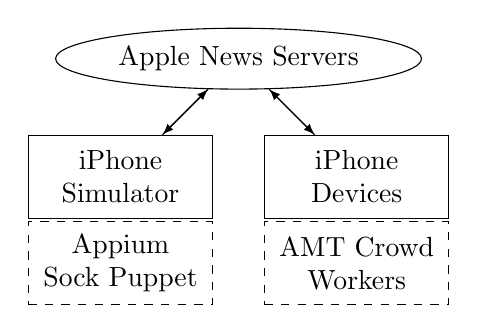
\begin{tikzpicture}[node distance = 2cm, auto]
    % Place nodes
    \node [cloud] (init) {Apple News Servers};
    \node [below of=init,node distance=1.5cm] (dummy) {};
    \node [block, left of=dummy,node distance=1.5cm] (sim) {iPhone Simulator};
    \node [block, right of=dummy,node distance=1.5cm] (dev) {iPhone Devices};
    \node [dashblock, below of=sim] (app) {Appium Sock Puppet};
    \node [dashblock, below of=dev] (amt) {AMT Crowd Workers};
    % Draw edges
    \path [line] (init) -- (sim);
    \path [line] (sim) -- (init);
    \path [line] (init) -- (dev);
    \path [line] (dev) -- (init);

\end{tikzpicture}
    \caption{A depiction of our two audit methods: crowdsourced auditing via Amazon Mechanical Turk workers, and sock puppet auditing via an Appium-controlled iPhone simulator.}
    \label{fig:my_label}
\end{figure}


\subsection{Mechanism Audit}

\subsubsection{Experiment 1a: Measuring platform-wide update frequency.}\label{platform-wide}
We identify two content update mechanisms on Apple News: platform-wide updates and user-specific updates. In platform-wide updates, the ``master list'' of Trending Stories changes on the Apple News servers. The two types of updates may not always correlate: an update to the master list may not cause an update to the stories seen by a given user. We tested the platform-wide update frequency by continually checking for new content and measuring how often content changed. In this experiment, we set Apple News to not use any personalization data from other apps by turning off the ``Find Content in Other Apps'' toggle in the settings. We also removed files from the app's cache folder before every refresh. These measures were intended to minimize any potential content adaptation while we investigated the platform-wide update frequency of the Trending Stories section. However, the measures took time to perform, as did the process of opening the app, locating the buttons, and pressing the buttons via Appium. Thus, the maximum frequency with which we could record Trending Stories this way was approximately every 2 minutes.

\subsubsection{Experiment 1b: Measuring user-specific update frequency.}\label{user-specific}
Our initial experiment to test for user-specific update frequency happened by accident when we collected data for 12 continuous hours without closing the app and observed no changes in the Trending Stories. This led us to ask: Under what conditions does Apple News allow new Trending Stories from the ``master list'' to populate a user's app? In other words, what might be the user-specific update frequency? To answer this, we performed the same process as in experiment 1a, continuously collecting data from the app, but \textit{without deleting the cache and user identification files}. This allowed us to determine whether Apple News updates Trending Stories on a different schedule for individual users compared to the ``master list.''


\subsubsection{Experiment 2: Testing for location-based adaptation.}
While Apple News is known to adapt stories at a national level \citep{Brown2018}, we wondered whether stories changed with respect to a more fine-grain measure of location such as city or state. To test for fine-grain localization, we designed an experiment to elicit differences in content that could be accounted for by differences in a device's location.

In this experiment, we gathered stories from different simulated locations via Appium. Because it was not possible to run 50 simulators in parallel, we designed a way to sequentially collect and analyze data for evidence of localization, while still controlling for differences owed to time. We ran two iPhone simulators in parallel: one control, and one experimental. The control simulator was virtually located at Apple's headquarters and collected a set of control headlines, while the experimental simulator was virtually moved around the country to the 50 state capitals to collect local headlines in each place. Both simulators collected all Trending Stories shown in the app. We defined location-based adaptation (i.e. localization) as local headlines differing from  control headlines at a single point in time. Algorithm \ref{localization_algorithm} details the experiment.

\begin{algorithm}
\caption{Check for localization via sock-puppeting}\label{localization_algorithm}
\begin{algorithmic} 
\REQUIRE{set of locations $L$, $control\_location$}
\STATE set control simulator location to $control\_location$
\FOR{each $location$ in $L$}
\STATE set experimental simulator location to $location$
\STATE collect $local\_headlines$ and $control\_headlines$
\IF{$control\_headlines$ != $local\_headlines$}
\RETURN True \COMMENT{control headlines differed from local headlines, thus localization}
\ENDIF
\ENDFOR
\RETURN False \COMMENT{No localization observed}
\end{algorithmic}
\end{algorithm}

\subsubsection{Experiment 3: Measuring user-based adaptation.}
Location is one variable that might be used to adapt content across users. However, in Apple News, individual users can ``follow'' specific topics and publishers. This feature is used to populate the app with personalized content outside of the Trending Stories and Top Stories sections, but it is unclear whether it may also be used to adapt stories in the Trending Stories section. Because of the social and political implications of personalizing content, we wanted to test whether any personalization was applied to the algorithmically-curated Trending Stories section -- we do not examine Top Stories for personalization because Apple's editorial team is known to ``select five stories to lead the app'' in the United States \citep{Nicas2018}. In the personalization experiment, we used AMT to collect synchronized user screenshots, and compared the list of headlines to a control list that we collected concurrently from the simulator (which contained no cache files or user profile data).

Meaningful quantitative comparison of ranked lists is nontrivial. As \cite{Webber2010} point out, ``testing for statistical significance becomes problematic,'' since ``any finding of difference'' disproves a null hypothesis that rankings are identical. Researchers have therefore proposed and used various metrics to quantify the \textit{degree} of similarity between ranked lists, depending on the characteristics of the list. For example, rank-biased overlap (RBO) is designed for lists in which (1) the length is indefinite and (2) items at the top of the list are more important than items in the tail \citep{Webber2010}, and can be useful, for example, to investigate the degree of personalization in search engines  \citep{Robertson2018a}. 

While the Top Stories and Trending Stories lists vary in length across devices, their lengths are not ``indefinite'' since there is a known maximum length. Further, the weighting schemes in metrics such as RBO do not conceptually fit our data. This is because, as previously mentioned, one subset of Trending Stories (\#1-2) is displayed on iOS home screens, one subset (\#1-4) is shown within the app on all devices, and the full set of Trending Stories (\#1-6) is shown within the app on devices with large screens. Thus, a headline moving \textit{between} these subsets (ex. from \#5 to \#4) has more significant implications because the change will more substantively affect visibility compared to a headline moving \textit{within} a subset (e.g., from \#4 to \#3).

We therefore define user-based adaptation as a unique \textit{set} of stories appearing to a given user, quantified by the overlap coefficient (Szymkiewicz-Simpson coefficient)  \citep{Vijaymeena2016} between a user's Trending Stories and the Trending Stories on a control device. The overlap coefficient is a slight modification of Jaccard index, which is also used by \citet{Hannak}, \citet{Kliman-Silver2015}, \citet{Vincent2019}, and other studies to measure personalization in web search results. It operationalizes the definition of user-based adaptation as the size of the intersection divided by the smallest size of the two sets, and ranges from 0 (no overlap between sets) to 1 (one set includes all items in the other set). One key benefit of the metric is that it conceptually accommodates data from devices with smaller screens that showed only four Trending Stories, since our control list was on a large device and showed six Trending Stories.


\subsection{Content Audit}

\subsubsection{Experiment 4: Extended data collection.}
Finally, we designed and performed an extended data collection using Appium based on findings from the first three experiments. Each data point included a timestamp and a list of shortened URLs to the news stories, gathered by a simulated user tapping ``Share'' then ``Copy'' on each headline. To analyze the stories, a Python script followed each shortened URL along redirects until it reached a final web address, where it parsed the web page for a story title. The domain of the final address identified the publisher of the story (e.g. \texttt{cnn.com}).

%The URLs include a 23-character hash value, preceded by  \texttt{https://apple.news/}.

We compared the Top Stories and Trending Stories according to the update schedule, source diversity, and headline content. To quantify source diversity, we relied on the Shannon diversity index \citep{Shannon1948}, a metric which accounts for both abundance and evenness of different categories in a sample and derives from the probability that two randomly-chosen items belong to the same category (in our case, the same news source). Normalizing this value (dividing it by the maximum possible Shannon diversity index for the population) provides the Shannon \textit{equitability} index, also known as Pielou's index \citep{Pielou1966}, a more interpretable value between 0 and 1 where 1 indicates that all sources appeared with the same relative frequency (e.g., 50\% of Trending Stories from Fox and 50\% of Trending Stories from CNN). To statistically compare the source diversity of the Trending Stories section with that of the Top Stories section, we use the Hutcheson t-test \citep{Hutcheson1970}, which was specifically designed to compare the Shannon diversity index between two samples (in our case, the Trending Stories and the Top Stories).

%We tally the total number of stories appearing from each individual source and calculate the mean, median, standard deviation, and relative distribution of stories across all sources. We also calculate the amount of time each story spends in a given section (which can further characterize source concentration), as well as the total time each source was featured, the overall average duration stories were featured, and the source-specific average duration.

To compare content between the two sections, we first create a corpus of all headlines from Top Stories, and another corpus of all headlines from Trending Stories. We then count bigrams and trigrams within each set of headlines. Before doing this, each headline is stripped of punctuation and stopwords, then tokenized into bigrams and trigrams. We calculate the log ratio \citep{Hardie2014} of each n--gram to determine which are most salient relative to the other section.

%first stripped of punctuation, then tokenized using the nltk python package \citep{Bird2016a}. Finally, the bigrams from each headline are tallied into an aggregate table, which we manually filter for repetitive phrases and stopwords such as ``the'', ``is,'' ``and,'' etc.


\section{Results}
We now describe the results of our comparison between the HIGHLIGHTS strategy summarization method and our novel \disalg~ approach. We report the main experimental results with respect to the hypotheses raised in the previous section. 

Figure \ref{fig: DA HL compare} shows the percentage of participants who were successful in answering the experiment tasks in each of the experiment conditions, for each agent pair combination.

\emph{(H1) Participants in the HIGHLIGHTS condition struggled to successfully identify the better
performing agent in the comparison task.} When all agents are of decent performance, we see the difficulty
of distinguishing between them manifest itself in a poor success rate.
Based on participants' textual explanations of the choice of agent, it seems they were concerned that agent $E$ was indecisive, e.g., ``[Agent $E$] seems very indecisive while ... [Agent $M$] seems to have a plan and is going with it.''. %,  ``... [Agent $E$] behaved more like a human.''
We hypothesize that these responses are a consequence of a single trajectory in agent $E$'s summary where the frog is seen leaping between logs in a seemingly indecisive manner. These results emphasize the limitations of independent comparisons.
% summaries and strengthen our claims regarding their limitations.
% \ya{changed, but didn't mention anything regarding a random guess, not sure it's necessary}

% A Bootstrap analysis shows that in such a case,
% selecting the better performing agent is \emph{not} significantly different from a random guess  ($p > 0.59$ for all agent pairs).

% with  $(p =
% 0.59)$ for $E$ vs. $LV$, $(p = 0.595)$ for $E$ vs. $M$ and $(p = 0.595)$ for $LV$ vs. $M$. 

\emph{(H2) Participants in the \disalg~ condition were more successful in the agent comparison
task}. Participants in the \disalg~ group 
% given the same agents to compare, 
showed vast improvement
in the ability to identify the better performing Frogger agent  (see Figure \ref{fig: DA HL compare}). The differences in success rate between conditions  were statistically significant and  
substantial for all agent comparisons ($E$ vs. $LV$: $p = 1.6^{-5}$; $E$ vs. $M$: $p = 1.7^{-5}$; $LV$ vs. $M$: $p = 0.018$). Textual explanations provide insights regarding how the
contrastive nature of the \disalg~ summaries helped participants decide which agent to choose, e.g. `` I preferred the path that ... [Agent $E$] was taking''; ``I felt that ... [Agent $E$] was making slightly stronger moves, and pushing ahead further''.



% Figure \ref{fig: DA HL compare} reports the comparison in the percentage of participants that were
% able to correctly identify the better performing agent between the HIGHLIGHTS and \disalg~ summary
% methods. Participants observing the HIGHLIGHTS summaries showed poor success results for comparing
% between agents $E$ and $LV$, strengthening our H1 hypothesis -- \emph{Participants shown
% HIGHLIGHTS summaries of low-varying performance agents were not always able to correctly select
% the most skilled agent.} Participant in the \disalg~ group, given the same agents to compare,
% showed vast improvement in the ability to identify the better agent, strengthening our H2
% hypothesis -- \emph{Participants shown Disagreement summaries of low-varying performance agents
% were able to correctly select the most skilled agent.} The analysis shows a statistically
% significant and substantial difference in performance when comparing \disalg~ to HIGHLIGHTS with
% $(p < 1.4^{-5})$ for $E$ vs. $LV$ and $(p < 0.15)$ for $E$ vs. $HV$.

% \ya{maybe add some of the user study comments} \oa{yes, it would be nice if you could show an
% example comment or two from DA participants that shows the direct comparison helped them}


% \begin{itemize}
% 	\item \textbf{`` I preferred the path that ... was taking''} 
% 	\item \textbf{`` I felt that ... was making slightly stronger moves, and pushing ahead
% 	further''} 
% 	\item \textbf{``Agent ... was clearly making better choices''}
% \end{itemize}
%%%other options:
% ``Agent two made better choices overall in both videos''
% ``Agent 2 made smarter moves as a whole''
% ``Agent one got himself dead in the second video, the choice is easy.''
% ``Agent..reached lily pad first... further ahead first..''



% The analysis shows statistically significant and substantial differences in performance when
% comparing user success percentage using \disalg~ compared to HIGHLIGHTS. \ref{fig: DA HL compare}


% \emph{(H1) Participants shown HIGHLIGHTS summaries of low-varying performance agents were not
% always able to correctly select the most skilled agent.}  Participants’ selection for this agent
% comparison task are shown in Figure \ref{fig: HL vote}. These results support H1. The graphs
% indicate an agreement between our study participants that agent $LV$ dominates agent $E$ which we
% know to be false. A likely cause of this outcome can simply be the different states each agent
% determines as important, which results in different summary trajectories shown. This strengthens
% our claims regarding the limitations of HIGHLIGHTS summaries for comparison tasks due to
% non-dependency between the agents. 


% \begin{figure}[ht] \centering \includegraphics[width=0.75\columnwidth]{images/HL_hard_vote.png}\\
%   \vspace{-0.7cm} \caption{Agent selection using HIGHLIGHTS with low-varying performance agents}
%   \label{fig: HL vote} \vspace{-0.2cm} \end{figure}


% \emph{(H2) Participants shown Disagreement summaries of low-varying performance agents were able
% to correctly select the most skilled agent.}  Participants’ selection for this agent comparison
% task are shown in Figure \ref{fig: DA HL compare}. These results support H2. Given the same agents
% to compare, we can see a vast improvement in the user's ability to identify the better agent. 




% \begin{figure}[ht] \centering \includegraphics[width=0.75\columnwidth]{images/DA_vote.png}\\
%   \vspace{-0.7cm} \caption{Agent selection using the \disalg~ algorithm on low-varying
%   performance} \label{fig: DA vote} \vspace{-0.2cm} \end{figure}

% \begin{figure}[ht]
% 	\centering
% 	\includegraphics[width=0.75\columnwidth]{images/success.png}\\
% 	% \vspace{-0.7cm}
% 	\caption{Agent selection success percentage}
% 	\label{fig: DA HL compare}
% % 	\vspace{-0.2cm}
% \end{figure}

\emph{(H3) A significant difference was found between success rates of participants in the conveying differences task}. Participants achieved a significantly higher success rate with the \disalg~ method in the $FR$ vs. $SD$ comparison ($p = 0.014$). Albeit, this was mostly a result of the low performance of HIGHLIGHTS in $Q1$ due to the $SD$ summary containing, coincidentally, only trajectories of the agent at the bottom lane. 
The inferior performance of \disalg~ in $Q1$ of $CL$ vs. $FR$  ($p = 0.187$) can be explained by summary trajectories where no vehicles were present in $CL$'s lane allowing it to drive faster than $FR$ and appear less considerate of keeping distance.
While not necessarily outperforming it, the \disalg~ is at least equivalently useful as HIGHLIGHTS, which was shown to be better than random~\cite{Tobias}.


% \emph{(H3) Explanation satisfaction of participants shown \disalg~ summaries was similar to that of
% participants shown HIGHLIGHTS summaries.} Participants’ distributions of scores for the explanation
% satisfaction were not statistically significant $(p_{exp\#1} = 0.17, p_{exp\#2} = 0.61)$.

\emph{(H4) No clear participant preference towards one summary method was observed.} Most participants answered that both methods were equally beneficial. However,
more participants found \disalg~ more \emph{helpful} and containing less irrelevant information than HIGHLIGHTS, while finding the latter more \emph{pleasing}.



% \begin{figure}[ht]
% 	\centering
% 	\includegraphics[width=0.65\columnwidth]{images/sat.png}\\
% % 	\vspace{-0.7cm}
% 	\caption{User satisfaction of summary methods}
% 	\label{fig: sat}
% % 	\vspace{-0.2cm}
% \end{figure}

% \emph{Confidence of correct participants.}
% Figure \ref{fig: conf}  shows the confidence
% ratings of participants who made the correct choice.\footnote{We compare the confidence ratings of
% correct participants, as being confident in a wrong choice is not desirable.} Ratings were slightly higher in two of the comparisons for the \disalg~ condition, however, none of the differences were statistically significant. 
% The analysis shows $(p = 0.68)$ for $E$ vs. $LV$, $(p  = 0.08)$ for $E$ vs. $M$ and $(p = 0.15)$ for $LV$ vs. $M$. 

\emph{Confidence and satisfaction}
In both experiments no statistically significant differences were found between the confidence or satisfaction of participants in different conditions (See Appendix).



% \emph{Correct participants in the \disalg~ condition were more confident than correct participants
% in the HIGHLIGHTS condition.} In addition to the agent selection success rate metric, we measured
% participants’ confidence in their selections. Figure \ref{fig: conf}  shows the confidence ratings
% of participants who made the correct choice\footnote{We compare the confidence ratings of correct
% participants, as being confident in a wrong choice is not desirable.}, showing that correct
% participants in the \disalg~ condition were more confident than correct participants in the
% HIGHLIGHTS condition. This difference was statistically significant for two of the three agent pairs
% ($(p < 0.017)$ for $E$ vs. $LV$ and $(p < 0.005)$ for $E$ vs. $HV$). 
% and the analysis show an increase in confidence of participants exposed to the \disalg~ summaries,
% with $(p < 0.017)$ for $E$ vs. $LV$ and $(p < 0.005)$ for $E$ vs. $HV$.


% \begin{figure}[ht]
% 	\centering
% 	\includegraphics[width=0.65\columnwidth]{images/conf.png}\\
% 	% \vspace{-0.5cm}
% 	\caption{Confidence of correct participants}
% 	\label{fig: conf}
% % 	\vspace{-0.2cm}
% \end{figure}


\vspace{-0.5em}
\subsection{Discussion}
In this section, we analyze the results from the study and provide examples of the 4 scenarios in Section \ref{sec:corgi} that we encountered. As hypothesized, scenario $\mathfrak{A}$ 
% (users not knowing the answer) 
hardly occurred as the commands are about day-to-day activities that all users are familiar with.
% Since our domain is concerned with commonsense knowledge about day-to-day activities, scenario $\mathfrak{A}$ (users not knowing the answer) hardly occurred. \amoscomment{This exact sentence appeared earlier (in the method section). Either remove or at least add "as mentioned / stated" or maybe "as hypothesized" (assuming the next sentence strengthens this)?}
% We did not observe any meaningful correlation between the student's background and their success rate, which is expected since the reasoning tasks are in the context of day-to-day activities. \amoscomment{What do you mean by "student's background", did you measure Pearson's correlation? What exact values did you get? I would recommend just removing this sentence due to lack of space.}
% Let us now discuss why CORGI is not able to achieve
% our observations of the study's dialog transcript and explain why there is a 
% ideal performance in the oracle scenario. This is mainly caused by the inability to extract the relevant knowledge from the human subjects, and partly caused by the limitations of the parser. 
% Scenario $\mathfrak{B}$ refers to cases where users misunderstood the question.
We did encounter scenario $\mathfrak{B}$, however. The study's dialogs show that some users provided means of \emph{sensing} the \textGoal rather than the \emph{cause} of the \textGoal.
% provided the meaning of certain queries rather than commonsense knowledge.
For example, for the reasoning task \emph{``If there are thunderstorms in the forecast within a few hours then remind me to close the windows because I want to keep my home dry''}, in response to the system's prompt \emph{``How do I know if `I keep my home dry'?''} a user responded \emph{``if the floor is not wet''} as opposed to an answer such as \emph{``if the windows are closed''}. Moreover, some users did not pay attention to the context of the reasoning task. For example, another user responded to the above prompt (same reasoning task) %Amos: I recommend removing "same reasoning task"
with \emph{``if the temperature is above 80''}! %Amos: This is an excellent paragraph!
% which is not even correct common sense (except perhaps in certain climates). 
Overall, we noticed that CORGI's ability to successfully reason about an if-then-because statement was heavily dependent on whether the user knew how to give the system what it needed, and not necessarily what it asked for; see Table \ref{tab:dialog} for an example. As it can be seen in Table \ref{tab:user_study}, expert users are able to more effectively provide answers that complete CORGI's reasoning chain, likely because they know that regardless of what CORGI asks, the object of the dialog is to connect the because \textGoal back to the knowledge base in some series of if-then rules (\textGoal/sub-\textGoal path in Sec.\ref{sec:corgi}). Therefore, one interesting future direction is to develop a dynamic context-dependent Natural Language Generation method for asking more effective questions.
% In contrast, CORGI's current method of asking, ``How do I know if \textGoal?'' often mis-states the immediate information need of the system. If users are not prompted with a good question, they cannot be expected to provide useful answers to the system. Therefore, one interesting future direction is to develop a dynamic context-dependent Natural Language Generation method for asking more effective questions. 
%This can be addressed by asking more informative questions that help users to consider the context in their answers. In the future, we will develop dynamic context-dependent Natural Language Generation pipelines to address this. % For example, instead of asking ``how do I know if $\textGoal$'', CORGI could ask, ``what does the $\textAction$ cause that allows you to achieve the $\textGoal$ ?''.

We would like to emphasize that although it seems to us, humans, that the previous example requires very simple background knowledge that likely exists in SOTA large commonsense knowledge graphs such as ConcepNet\footnote{\url{http://conceptnet.io/}}, ATOMIC\footnote{\url{https://mosaickg.apps.allenai.org/kg_atomic}} or COMET \cite{bosselut2019comet}, this is not the case (verifiable by querying them online). 
% Even the generative COMET model \cite{bosselut2019comet} is not able to generate commonsense knowledge relevant to this reasoning task. 
For example, for queries such as \emph{``the windows are closed''}, COMET-ConceptNet generative model\footnote{\url{https://mosaickg.apps.allenai.org/comet_conceptnet}} returns knowledge about blocking the sun, and COMET-ATOMIC generative model\footnote{\url{https://mosaickg.apps.allenai.org/comet_atomic}} returns knowledge about keeping the house warm or avoiding to get hot; which while being correct, is not applicable in this context. For \emph{``my home is dry''}, both COMET-ConceptNet and COMET-ATOMIC generative models return knowledge about house cleaning or house comfort. On the other hand, the fact that 40\% of the novice users in our study were able to help CORGI reason about this example with responses such as \emph{``If I close the windows''} to CORGI's prompt, is an interesting result. This tells us that conversational interactions with humans could pave the way for commonsense reasoning and enable computers to extract just-in-time commonsense knowledge, which would likely either not exist in large knowledge bases or be irrelevant in the context of the particular reasoning task.  
% Overall, the success rate of reasoning for this statement was $40\%$ i.e. 18 out of the 45 user interactions for this statement succeeded. %\facomment{make it more precise}.
% \tmcomment{maybe delete next two sentences to save space?} We would like to add that a comprehensive analysis of the performance of these large knowledge bases requires developing models targeted at solving our proposed reasoning task and is out of the scope of our current study. We hope instead, that this discussion reveals gaps in the commonsense reasoning literature to be addressed by the reasoning community's future endeavours.
Lastly, we re-iterate that as conversational agents (such as Siri and Alexa) enter people's lives, leveraging conversational interactions for learning has become a more realistic opportunity than ever before.
% \begin{figure}[t]
    \centering
    \resizebox{0.7\textwidth}{!}{
    \begin{tabular}{p{\columnwidth}}%{p{0.3\textwidth}}
    \toprule
    Successful task\\
    \midrule
    If it's going to rain in the afternoon then remind me to bring an umbrella because I want to remain dry.\\
    \hspace{2em}\textit{How do I know if ``I remain dry''?}\\
    If I have my umbrella.\\
    \hspace{2em}\textit{How do I know if ``I have my umbrella''?}\\
    If you remind me to bring an umbrella.\\
    \hspace{2em}\textit{Okay, I will perform ``remind me to bring an umbrella'' in order to achieve ``I remain dry''.}\\
    \\
    \toprule
    Failed task\\
    \midrule
    If it's going to rain in the afternoon then remind me to bring an umbrella because I want to remain dry.\\
    \hspace{2em}\textit{How do I know if ``I remain dry''?}\\
    If I have my umbrella.\\
    \hspace{2em}\textit{How do I know if ``I have my umbrella''?}\\
    If it's in my office.\\
    \hspace{2em}\textit{How do I know if ``it's in my office''?}\\
    ...
    \\
    \bottomrule
    \end{tabular}
    }
    \caption{Sample dialogs from our user study. CORGI's responses are noted in italics.}
    \label{fig:dialog}
\end{figure}

% \amoscomment{In the previous two scenarios you stated what they were. Either add it here as well, or if there isn't enough space, just remove and let the reader go back to section 3.1.} \facomment{sure, removed the previous ones, thanks}
In order to address scenario $\mathfrak{C}.1$, the conversational prompts of CORGI 
% Another point of failure for CORGI is caused by the fact that conversational prompts of the computer 
ask for specific small pieces of knowledge that can be easily parsed into a predicate and a set of arguments. However, some users in our study tried to provide additional details, which challenged CORGI's natural language understanding. 
% that some users gave all the reasoning steps in answer to the first question, which confused the parser. 
For example, for the reasoning task \emph{``If I receive an email about water shut off then remind me about it a day before because I want to make sure I have access to water when I need it.''}, in response to the system's prompt \emph{``How do I know if `I have access to water when I need it.'?''} one user responded \emph{``If I am reminded about a water shut off I can fill bottles''}. This is a successful knowledge transfer. However, the parser expected this to be broken down into two steps. If this user responded to the prompt with \emph{``If I fill bottles''} first, CORGI would have asked \emph{``How do I know if `I fill bottles'?''} and if the user then responded \emph{``if I am reminded about a water shut off''} CORGI would have succeeded. The success from such conversational interactions are not reflected in the overall performance mainly due to the limitations of natural language understanding.%, which we are planning to address in the future.

% The effectiveness of interactive reasoning and well as the learned rule embeddings is shown in Table \ref{tab:user_study}. 
Table \ref{tab:user_study} evaluates the effectiveness of conversational interactions for proving compared to the no-feedback model. The 0\% success rate there reflects the incompleteness of \KB. The improvement in task success rate between the no-feedback case and the other rows indicates that when it is possible for users to contribute useful common-sense %Amos: commonsense is usually written as one word in this paper.
knowledge to the system, performance improves. The users contributed a total number of 96 rules to our knowledge base, 31 of which were unique rules. 
Scenario $\mathfrak{C}.2$ occurs when there is variation in the user's natural language statement and is addressed with our neuro-symbolic theorem prover. Rows 2-3 in Table \ref{tab:user_study} evaluate our theorem prover (\emph{soft unification}). 
% and replaces the Neuro-Symbolic theorem prover in Fig \ref{fig:model} with different variations.
% in parallel with soft proving.
% CORGI's performance is a combination of both successful knowledge acquisition and successful soft logical proving. But  CORGI has a serial design, such that it can only succeed when both components succeed.
% The no-feedback scenario, in which we do not engage in a conversation with the user, compared with all the other rows reflect the incompleteness of the knowledge base and the need for missing knowledge acquisition. We address it here by conversing with the users. The other 3 rows evaluate the effectiveness of the learned rule embeddings.
% Hard unification 
% (row 2) uses vanilla Prolog for proving and depends on hard unification (i.e. exact matches) for predicates. Therefore, it 
% is not capable of supporting the variations of natural language.
% HARD HERE: Soft unification improves the performance of hard unification significantly, since the latter is not capable of supporting the variations of natural language. Oracle unification (row 4) results show that 
% is the performance of our inference algorithm (Alg.\ref{alg:inference}) when oracle rule and variable embeddings are available. 
Having access to the optimal rule for unification 
% at each step of the proof 
does still better, but the task success rate is not 100\%, mainly due to the limitations of natural language understanding explained earlier.  %However, this usually did not occur. %Amos: I removed this, I think that it is confusing. You can write "However, even when using oracle unification the majority of rules cannot be proven".

% %Some of the performance loss in Table~\ref{tab:user_study}, is due to an imperfect parser. Better parsing would let us extract predicate arguments in a more robust manner. % \kmcomment{identify types? extract phrases? something specific}.
% There are several other opportunities for exploring improvements to the system. 
% Extending CORGI to handle conjunction statements would let us cover more of the if-then-because scenarios from Table \ref{tab:statement_stats}. Furthermore, the rule embeddings are not currently updated as the user interacts with the model. While a successful dialog with the system does add new facts to the knowledge base as shown in Figure \ref{fig:model} (\emph{knowledge update loop}), a neural model that could adaptively update and add embeddings for new facts and rules on the fly would support handling \emph{future} statements that are semantically similar to the added rule. 

% \kmcomment{run the experiment for no-feedback so we can include denominators} \kmcomment{run an experiment without soft-unification} \amoscomment{Table 4 is in the Appendix, don't reference it here.}
%
%
%\begin{table}[t]
%    \centering
%    \begin{tabular}{ccc}
%    Statement & Novice & Expert \\\hline
%    CORGI total & 16/88 & 8/24  \\\hline
%%If I have an early morning meeting then wake me up early because I want to be ontime. 
%1 & 1 & 1 \\
%%If there are thunderstorms in the forecast within a few hours then remind me to close the windows because I want to keep my home dry. 
%2 & 3& 2  \\
%%If I schedule an appointment that overlaps with another appointment then notify me immediately because I want to let my colleagues know of the conflict. 
%3* & 0& 0 \\
%%If I search for a gas station in the navigation app and there is a cheaper gas station that is not too much further away then ask me immediately whether I want to switch the destination to the new gas station because I want to save money. 
%4 & 0& 0 \\
%%If I search for a restaurant in the navigation app and there is a cheaper restaurant with a similar rating then notify me immediately whether I want to switch the destination to the new restaurant because I want to save money. 
%5 & 0& 0 \\
%% If I receive an email about a critical software update then notify me immediately because I want to keep my computers safe from malware. 
%6 & 0& 0 \\
%%If it's going to rain in the afternoon then remind me to bring an umbrella because I want to remain dry.
%7* & 0& 0\\
%%If I haven't been to the gym for more than 3 days then remind me to go to the gym because I want to stay fit. 
%8 & 6 & 3  \\
%%If I receive an email about water shut off then remind me about it a day before because I want to make sure I have access to water when I need it. 
%9 & 0 & 0 \\
%%If my calender is clear today, then remind me to go to gym in the afternoon, because I want to keep myself healthy. 
%10 & 6 &2 \\
%    \end{tabular}
%    \caption{Percentage of users who were able to prove each statement in the target study set. *: These statements saw fewer proof attempts due to a bug in the initial round of tests.}
%    \label{tab:user_study}
%\end{table}

% \vspace{-1em}
\section{Conclusions}
% \vspace{-1em}
In this paper, we introduced a benchmark task for commonsense reasoning that aims at uncovering unspoken intents that humans can easily uncover in a given statement by making presumptions supported by their common sense. In order to solve this task, we propose
CORGI (COmmon-sense ReasoninG by Instruction),  a neuro-symbolic theorem prover that performs commonsense reasoning by initiating a conversation with a user. CORGI has access to a small knowledge base of commonsense facts and completes it as she interacts with the user. We further conduct a user study that indicates the possibility of using conversational interactions with humans for evoking commonsense knowledge and verifies the effectiveness of our proposed theorem prover.
% We defined common-sense reasoning as the process of finding a chain of reasoning in a logic program given an if/then/because statement. We showed that obtaining the because statement is crucial in extracting a relevant chain of reasoning given an if/then statement. Moreover, we introduced a soft backward chaining algorithm that allows us to combat variations in natural language by learning embeddings for the facts and rules in the knowledge base. This algorithm combines symbolic AI with neural approaches allowing us to bridge a gap between symbolic AI and the recent advances in deep learning.

\section{Acknowledgements}
This work is funded in part by the National Science Foundation under award number IIS-1717330.

\small{
\bibliography{library}
\bibliographystyle{aaai}
}
\end{document}